\documentclass[12pt, letterpaper]{article}
\usepackage[titletoc,title]{appendix}
\usepackage{color}
\usepackage{booktabs}
\usepackage[usenames,dvipsnames,svgnames,table]{xcolor}
\definecolor{dark-red}{rgb}{0.75,0.10,0.10} 
\usepackage[margin=1in]{geometry}
\usepackage[linkcolor=dark-red,
			colorlinks=true,
			urlcolor=blue,
			pdfstartview={XYZ null null 1.00},
			pdfpagemode=UseNone,
			citecolor={dark-red},
			pdftitle={Downweighting}]{hyperref}

\usepackage[resetlabels,labeled]{multibib}
\newcites{SI}{SI References}
\usepackage{natbib}

\usepackage{float}

\usepackage{geometry} % see geometry.pdf on how to lay out the page. There's lots.
\geometry{letterpaper}               % This is 8.5x11 paper. Options are a4paper or a5paper or other... 
\usepackage{graphicx}                % Handles inclusion of major graphics formats and allows use of 
\usepackage{amsfonts,amssymb,amsbsy}
\usepackage{amsxtra}
\usepackage{verbatim}
\setcitestyle{round,semicolon,aysep={},yysep={;}}
\usepackage{setspace}		     % Permits line spacing control. Options are \doublespacing, \onehalfspace
\usepackage{sectsty}		     % Permits control of section header styles
\usepackage{lscape}
\usepackage{fancyhdr}		     % Permits header customization. See header section below.
\usepackage{url}                     % Correctly formats URLs with the \url{} tag
\usepackage{fullpage}		%1-inch margins
\usepackage{multirow}
\usepackage{rotating}
\setlength{\parindent}{3em}

\usepackage[T1]{fontenc}
\usepackage{bm}
\usepackage{palatino}

\usepackage{chngcntr}

\def\citeapos#1{\citeauthor{#1}'s (\citeyear{#1})}

\makeatother


% Caption
\usepackage[hang, font=small,skip=0pt, labelfont={bf}]{caption}
%\captionsetup[subtable]{font=small,skip=0pt}
\usepackage{subcaption}

% tt font issues
% \renewcommand*{\ttdefault}{qcr}
\renewcommand{\ttdefault}{pcr}

\setcounter{page}{0}

\usepackage{lscape}
\renewcommand{\textfraction}{0}
\renewcommand{\topfraction}{0.95}
\renewcommand{\bottomfraction}{0.95}
\renewcommand{\floatpagefraction}{0.40}
\setcounter{totalnumber}{5}
\makeatletter
\providecommand\phantomcaption{\caption@refstepcounter\@captype}
\makeatother

\title{Explaining Partisan Affect: Partisan Response to Partisan Response}

\author{Douglas J. Ahler\thanks{Assistant Professor of Political Science, Florida State University, \href{mailto:dahler@fsu.edu}{\texttt{dahler@fsu.edu}}} \and Carolyn E. Roush\thanks{Democracy Postdoctoral Fellow, the Ash Center for Democratic Governance and Innovation at the Harvard Kennedy School, \href{mailto:carolyn_roush@hks.harvard.edu}{\texttt{carolyn\_roush@hks.harvard.edu}}}}

\begin{document}
\maketitle
\thispagestyle{empty}

\begin{abstract}

\noindent 

\end{abstract}

\newpage
\doublespacing

\section*{Study I: Partisan Response to Partisan Response to Scandals}

Does perception of the outparty as biased and unresponsive to political facts exacerbate affective polarization? Answering this question using observational data is difficult, primarily because partisans very rarely process information in an unbiased manner. As a result, it is near impossible to disentangle the effect of partisans' observation of out-party motivated reasoning from the effect of partisans' \textit{own} biased interpretation of facts or events. 

Accordingly, as a first test of our theory, we rely upon a randomized, controlled experiment to determine if and how partisans' exposure to out-party bias exacerbates the negative feelings they hold toward their opponents. Specifically, we use a series of vignettes about real political scandals and manipulate whether or not co-partisans responded to the scandal in an unbiased manner. This design holds constant both the scandal and the elite embroiled in the scandal, which helps to rule out important confounding variables that could muddle inferences drawn from observational data. Using this design, we can better assess whether partisans' (lack of) response to co-partisan elites' errors helps deepen partisan affect. 

In November 2013, we recruited 930 survey participants through Amazon's Mechanical Turk \citep[see][]{BerinskyHuberLenz2012}. To preclude suspicion, we told participants they would be participating in a broad survey on political media consumption and political learning. Prior to our experiment, we posed a question to determine whether or not respondents were paying attention to the survey. In particular, the question asked respondents to mark two particular responses. Of the 930 respondents, 38 respondents failed to complete the task as requested. We removed these participants from our sample as we felt that they were merely adding noise to the data. Because we are interested in \textit{partisans'} reactions to an observed response (or lack thereof) to out-party blunders, we further limit our analysis to responses from self-identified and leaning partisans.\footnote{We group together ``leaning'' Independents with ``strong'' and ``weak'' partisans, based on previous research suggesting Independent leaners think and behave similarly to partisans \citep{keithetal_1992}.} Of the 726 self-identified and leaning partisans, 552 are Democrats, consistent with the general liberal bias in MTurk samples \citep{BerinskyHuberLenz2012}. 

Participants were randomly assigned to read a news story on one of three contemporary political scandals: (1) the troubled rollout of the U.S. health exchange website, healthcare.org (which we classify as a Democratic Party scandal), (2) Senator Ted Cruz's controversial decision to force a government shutdown (which we classify as a Republican Party scandal), and (3) Toronto mayor Rob Ford's drug scandal (which we classify as a non-partisan scandal, thus representing our "control" condition). We selected these the Cruz and healthcare.gov cases because they were timely examples of real-world, high-profile missteps that generated significant news coverage. Within the non-control groups, we further manipulated whether Democratic (Republican) Party supporters' opinions of Obama (Cruz) changed in response to the blunder. This created five conditions based on vignette content:  (1) Obama - reponse, (2) Obama - no response, (3) Cruz - response, (4) Cruz - no response, and (5) control. (See Appendix A for vignettes.) After exposing respondents to these stories, we asked them to rate the Democratic and Republican parties using feeling thermometers. We use party feeling thermometer scores as our dependent variables in this study because they are the most common means by which to measure affective polarization \citep[e.g.,][]{haidthetherington_2012,hetheringtonrudolph_2015,IyengarSoodLelkes2012,iyengarwestwood_2014,mason_2015}. 

Though our sample is disproportionately Democratic, we analyze the results of our experiment separately among Democrats and Republicans to detect any partisan differences in response to the treatments. We also elect to analyze the feeling thermometers as separate dependent variables, as previous research demonstrates that the growing gulf in partisan affect has been caused primarily by increasing dislike of the out-party and not by a corresponding increase in warm in-party feelings \citep{haidthetherington_2012, IyengarSoodLelkes2012}. As out-party negativity is the prime mover over time, we might also expect our experiments to produce greater variation in the out-party feeling thermometers compared to the in-party feeling thermometers. Accordingly, our analysis produces four OLS regressions that analyze the impact of our experimental manipulation on out- and in-party affect among Democrats and Republicans. 

Table 1.1 presents the results of our experiment. For each model, we include four dummy variables representing assignment to our experimental conditions - (1) \textit{Out-Party - Response} (in which out-party supporters downgrade their evaluations of the co-partisan politician in response to the misstep), (2) \textit{Out-Party - No Response} (in which out-party supporters do not change their evaluations), (3) \textit{In-Party - Response} (in which the respondent's co-partisans downgrade their evaluations of an in-party politicians) and (4) \textit{In-Party - No Response} (in which the respondent's co-partisans do not change their evaluations).\footnote{\textit{Control} is the reference category.} Respondents are assigned a value of 1 if they were assigned to that particular condition and a value of 0 if they were not. The dependent variables --- the in- and out-party feeling thermometers --- range from 0 to 100. Positive coefficients indicate an increase in warmth toward the party in question; negative coefficients indicate a decrease in warmth toward the party in question.

\begin{spacing}{1}
\begin{table}
\begin{center}
\captionsetup{font={it}}
\caption{Party Affect by Experimental Condition}
\bigskip
\resizebox{\textwidth}{!}{
\begin{tabular}{lcccc} \hline
 & \multicolumn{2}{c }{{Republicans}} & \multicolumn{2}{c }{Democrats} \\ \hline \hline
  &  &  &  &  \\
 & Out-Party Affect & In-Party Affect & Out-Party Affect & In-Party Affect \\ \hline
 &  &  &  &  \\
Out-Party - Response & 6.640 & 8.991* & 0.428 & -6.026** \\
 & (5.409) & (4.943) & (2.799) & (2.749) \\
  &  &  &  &  \\
Out-Party - No Response & -0.972 & -2.880 & 1.222  & -2.635 \\
 & (5.409) & (4.943) & (2.970) & (2.918) \\
  &  &  &  &  \\
In-Party - Response & 2.942 & -3.337 & 2.920 & -5.317* \\
 & (5.190) & (4.744) & (2.848) & (2.798) \\
  &  &  &  &  \\
In-Party - No Response & -4.191 & 1.375 & 4.075 & -1.102 \\
 & (5.314) & (4.859) & (2.820) & (2.270) \\
  &  &  &  &  \\
Constant & 30.585*** & 63.171*** & 23.580*** & 68.010*** \\
 & (3.549) & (3.244) & (2.078) & (2.042) \\
 &  &  &  &  \\
Observations & 172 & 172 & 552 & 552 \\
 R-squared & 0.025 & 0.042 & 0.006 & 0.013 \\ \hline
&  &  &  &  \\
\multicolumn{5}{c}{ Standard errors in parentheses.} \\
\multicolumn{5}{c}{ ***\textit{p}$<$0.01, **\textit{p}$<$0.05, *\textit{p}$<$0.1, two-tailed.} \\
\end{tabular}}
\bigskip
\captionsetup{font={footnotesize,it}}
\caption*{Source: 2013 MTurk Study.}
\end{center}
\end{table}
\end{spacing}


\section*{Research Design, Study II: Partisan Response to Partisan Retrospective Evaluations}



\section*{Discussion and Conclusion}

\clearpage

\bibliographystyle{apsr}
\bibliography{xperceive}

\clearpage

\appendix
\renewcommand{\thesection}{A \arabic{section}}
\renewcommand\thetable{\thesection.\arabic{table}}  
\renewcommand\thefigure{\thesection.\arabic{figure}}
\counterwithin{figure}{section}

\begin{center}
\Large{Appendix}
\end{center}

\section{Study I Experimental Vignettes}

\begin{figure}[ht]
\centering
\begin{minipage}[b][12cm][b]{0.45\linewidth}
\caption{Obama - Response}
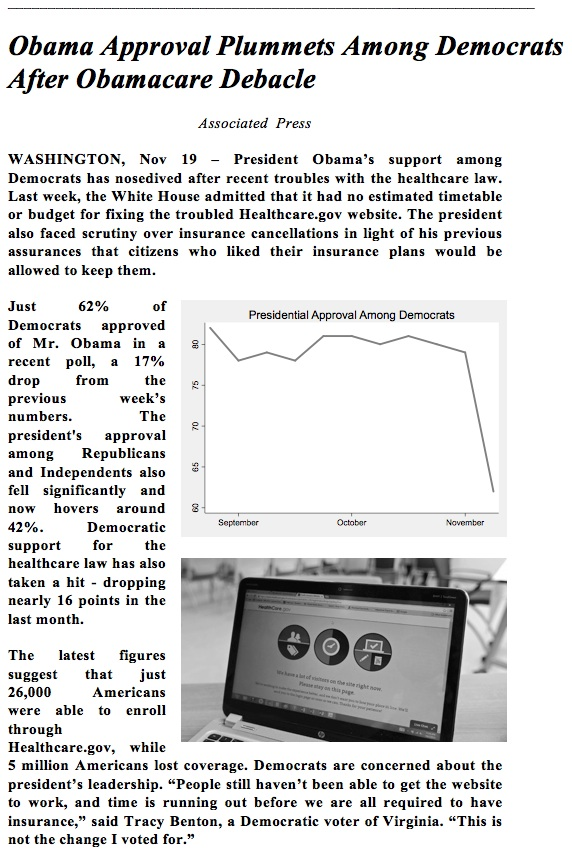
\includegraphics[width=1.05\textwidth]{Dem_C.jpg}
\label{fig:minipage1}
\end{minipage}
\quad
\begin{minipage}[b]{0.45\linewidth}
\caption{Obama - No Response}
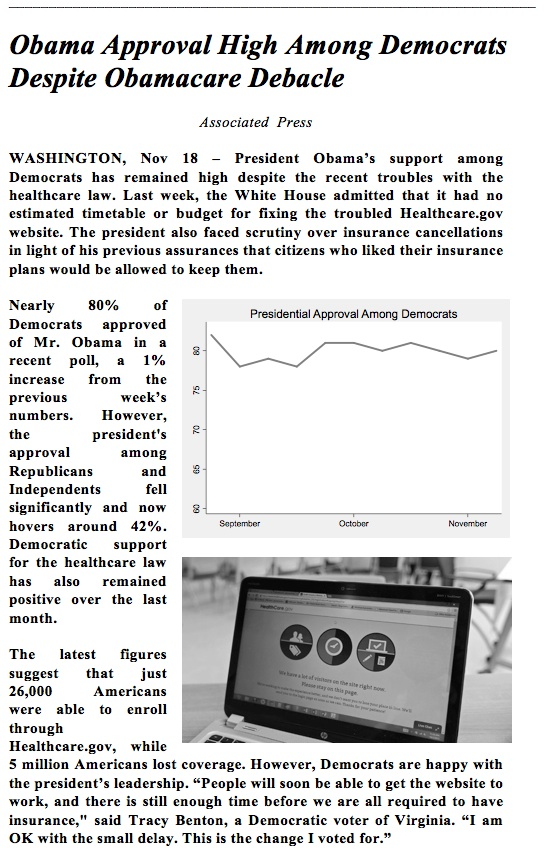
\includegraphics[width=1\textwidth]{Dem_T.jpg}
\label{fig:minipage2}
\end{minipage}
\end{figure}

\begin{figure}[ht]
\centering
\begin{minipage}[b][12cm][b]{0.45\linewidth}
\caption{Cruz - Response}
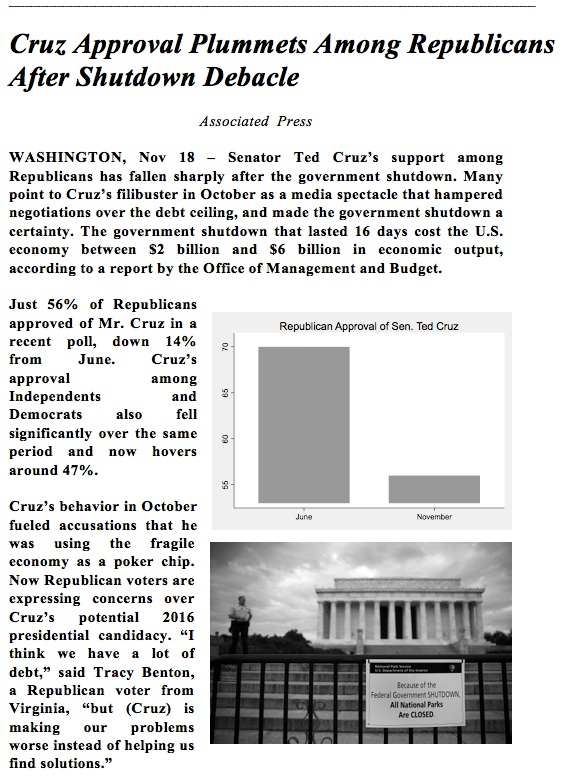
\includegraphics[width=1.05\textwidth]{Rep_C.jpg}
\label{fig:minipage3}
\end{minipage}
\quad
\begin{minipage}[b]{0.45\linewidth}
\caption{Cruz - No Response}
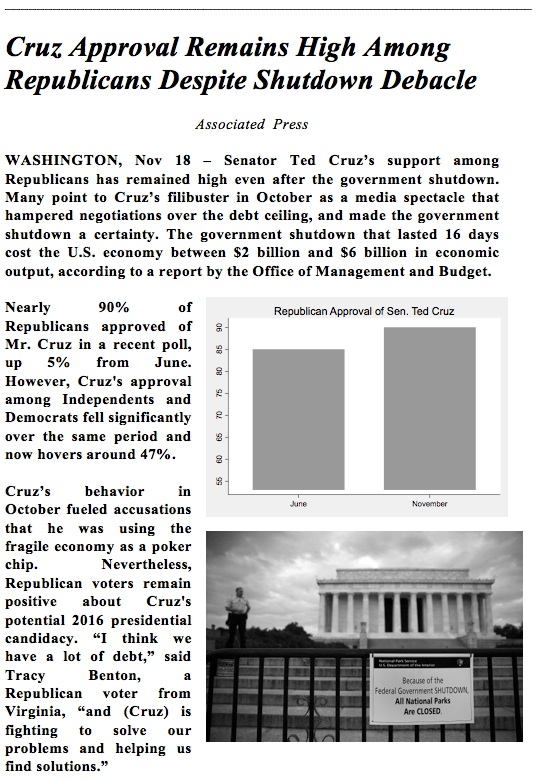
\includegraphics[width=1\textwidth]{Rep_T.jpg}
\label{fig:minipage4}
\end{minipage}
\end{figure}

\begin{figure}[ht]
\centering
\begin{minipage}[b][12cm][b]{0.45\linewidth}
\caption{Control}
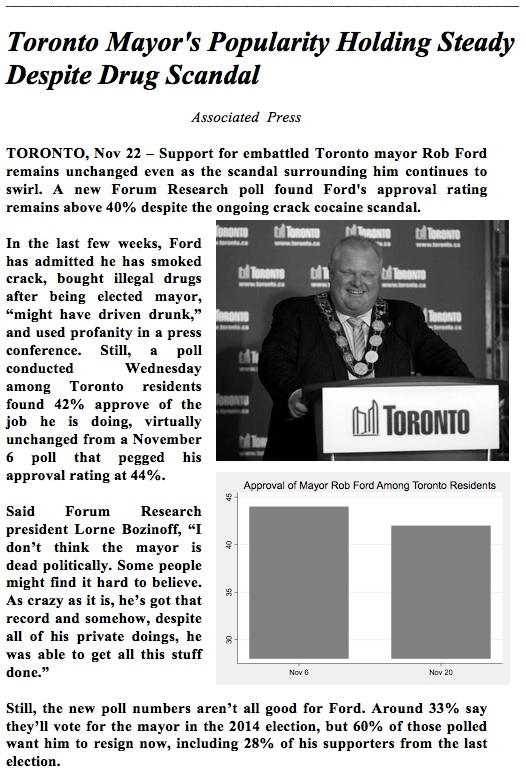
\includegraphics[width=1.05\textwidth]{P.jpg}
\label{fig:minipage5}
\end{minipage}
\end{figure}

\clearpage 

\section{Study II Experimental Vignettes}

\begin{figure}[ht]
\centering
\begin{minipage}[b][12cm][b]{0.45\linewidth}
\caption{Control}
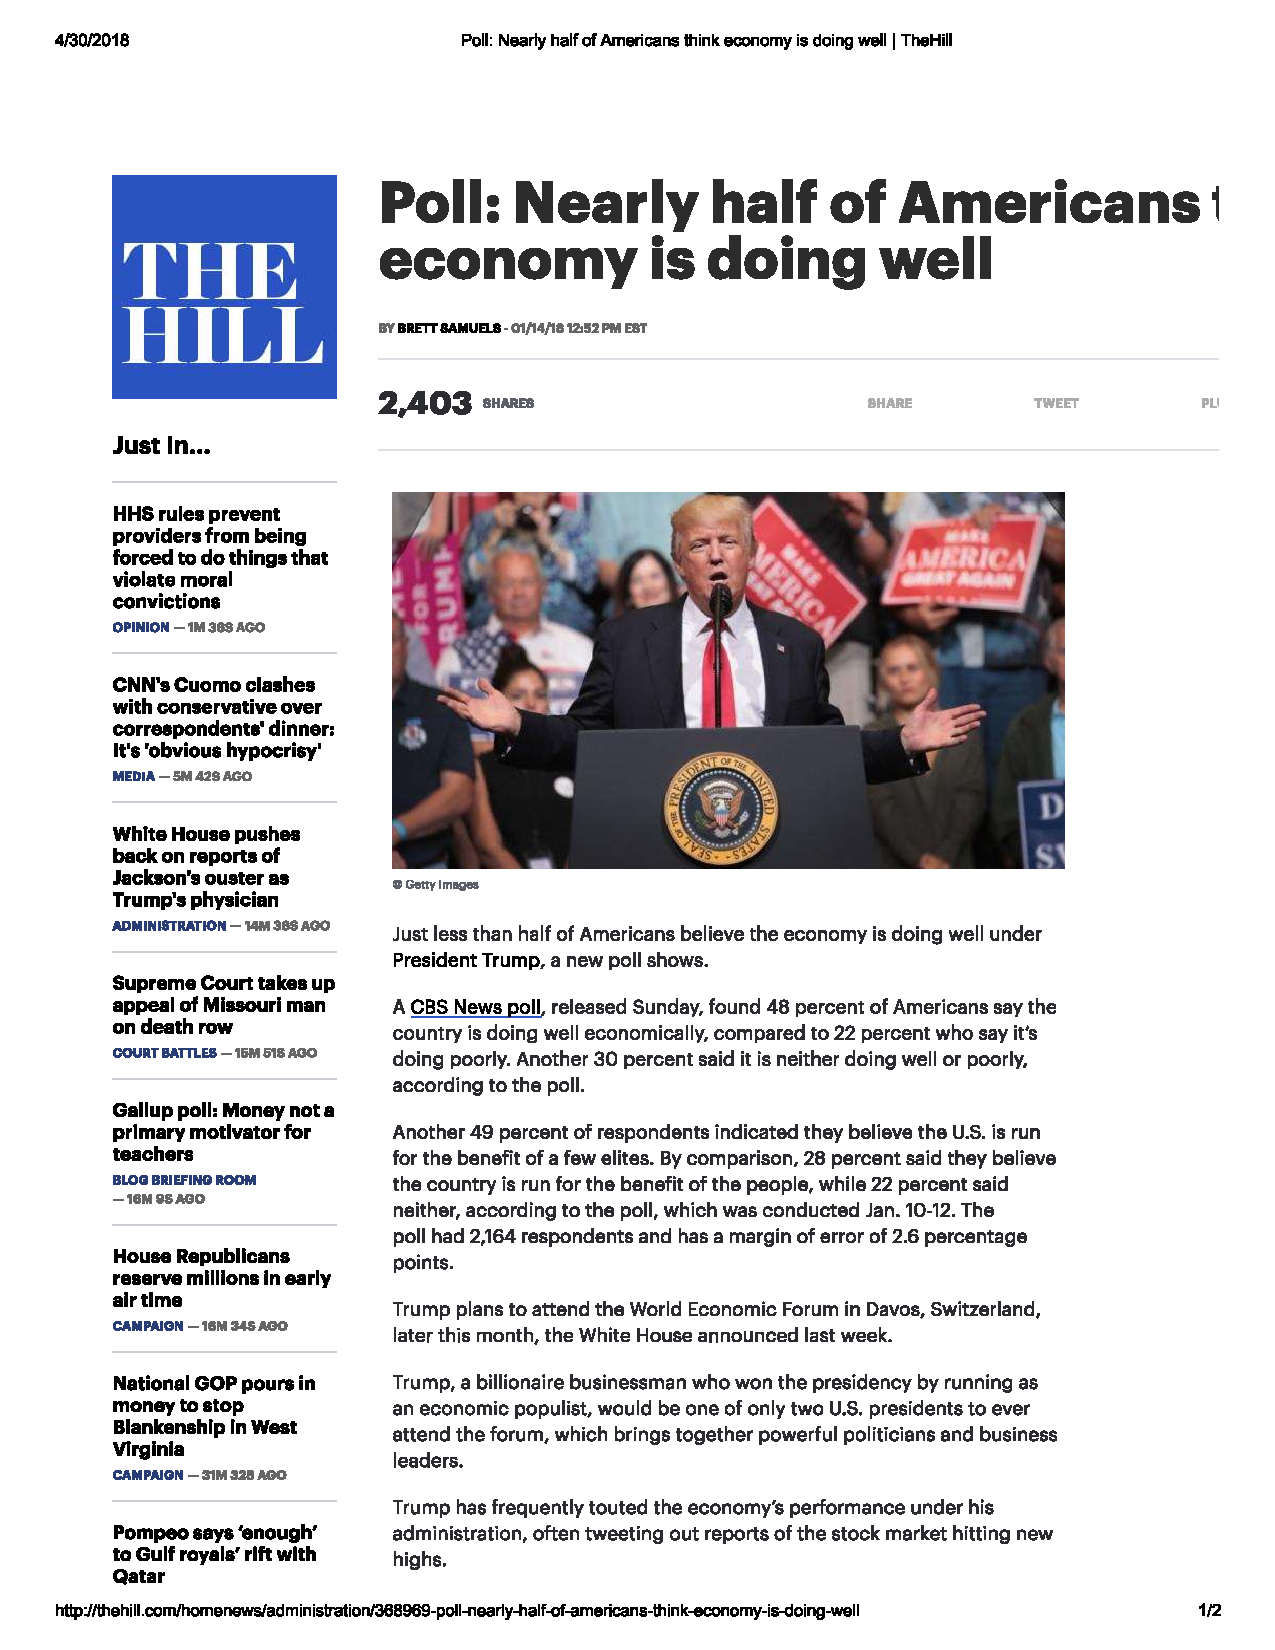
\includegraphics[width=1.05\textwidth]{control.pdf}
\label{fig:minipage3}
\end{minipage}
\quad
\begin{minipage}[b]{0.45\linewidth}
\caption{Bipartisan Bias}
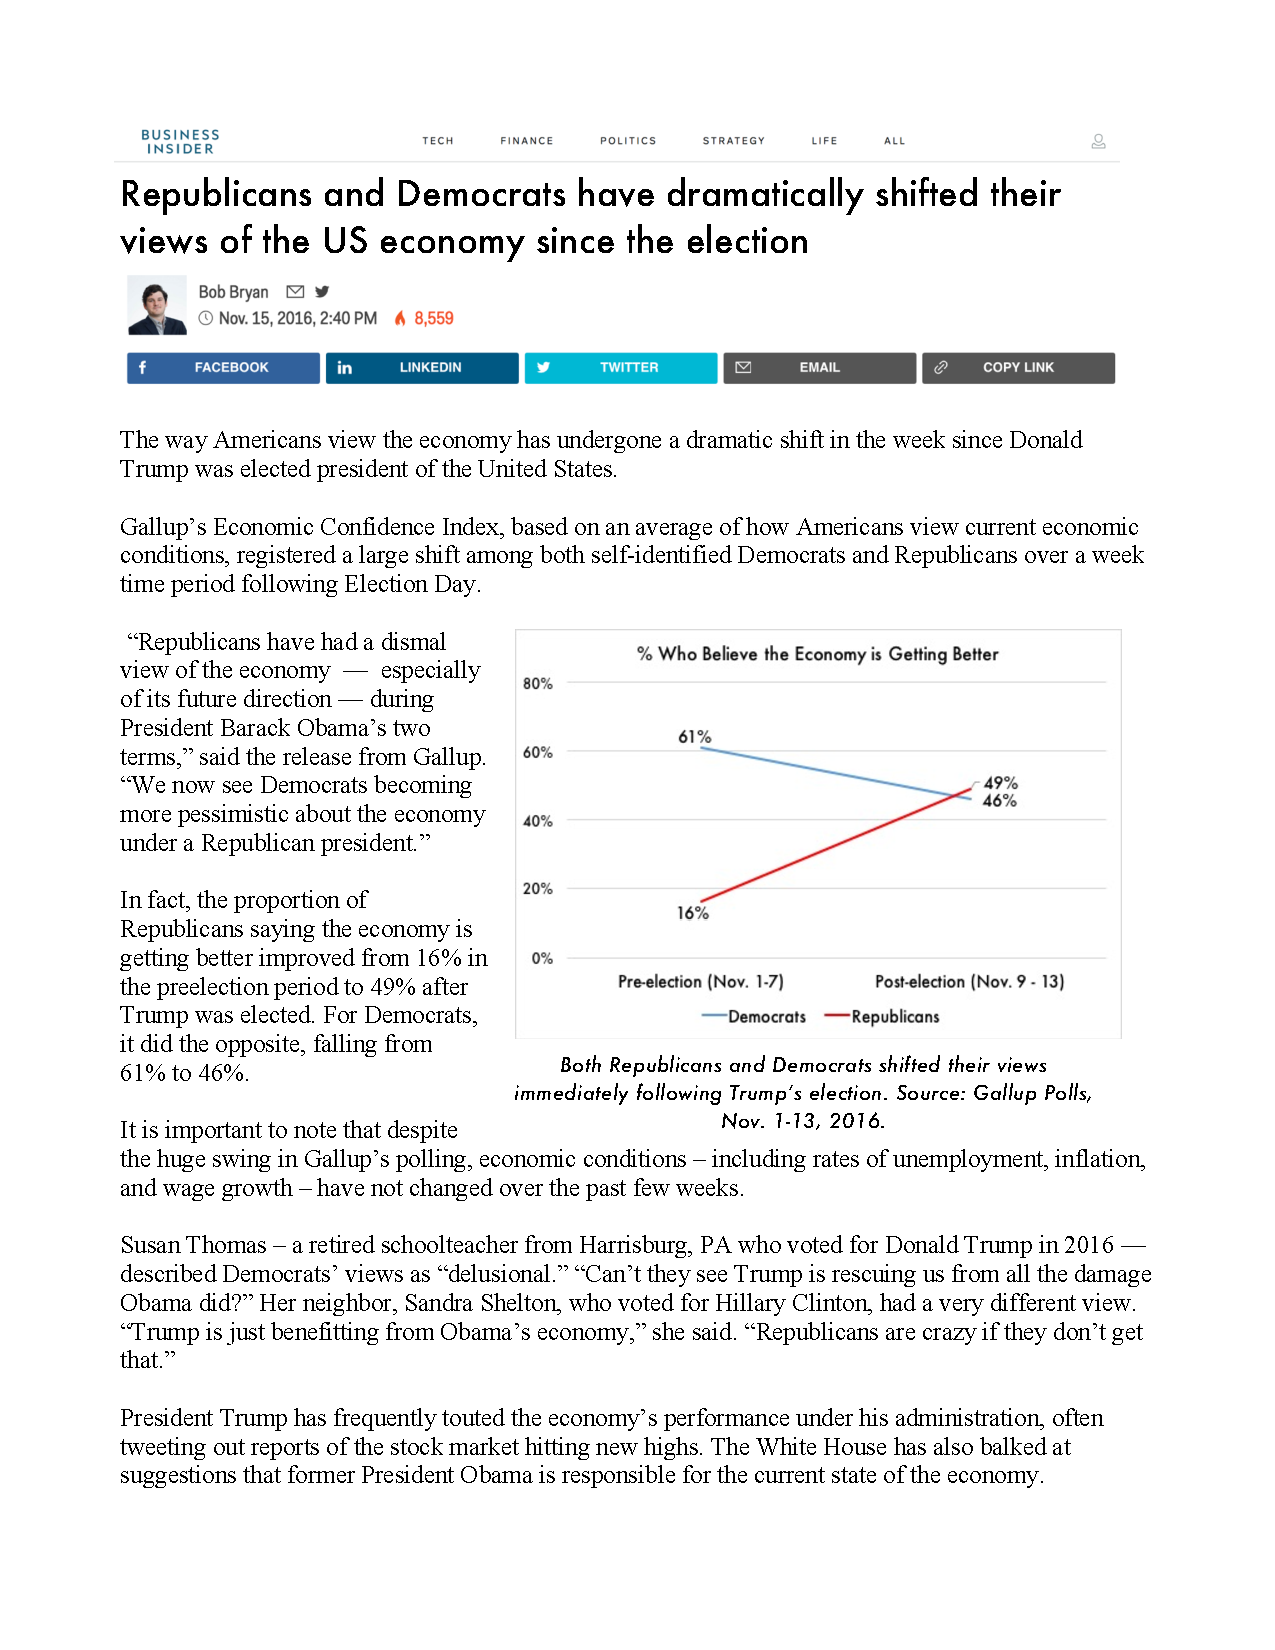
\includegraphics[width=1.05\textwidth]{bipart_motivate.pdf}
\label{fig:minipage4}
\end{minipage}
\end{figure}

\begin{figure}[ht]
\centering
\begin{minipage}[b][12cm][b]{0.45\linewidth}
\caption{Democratic Bias}
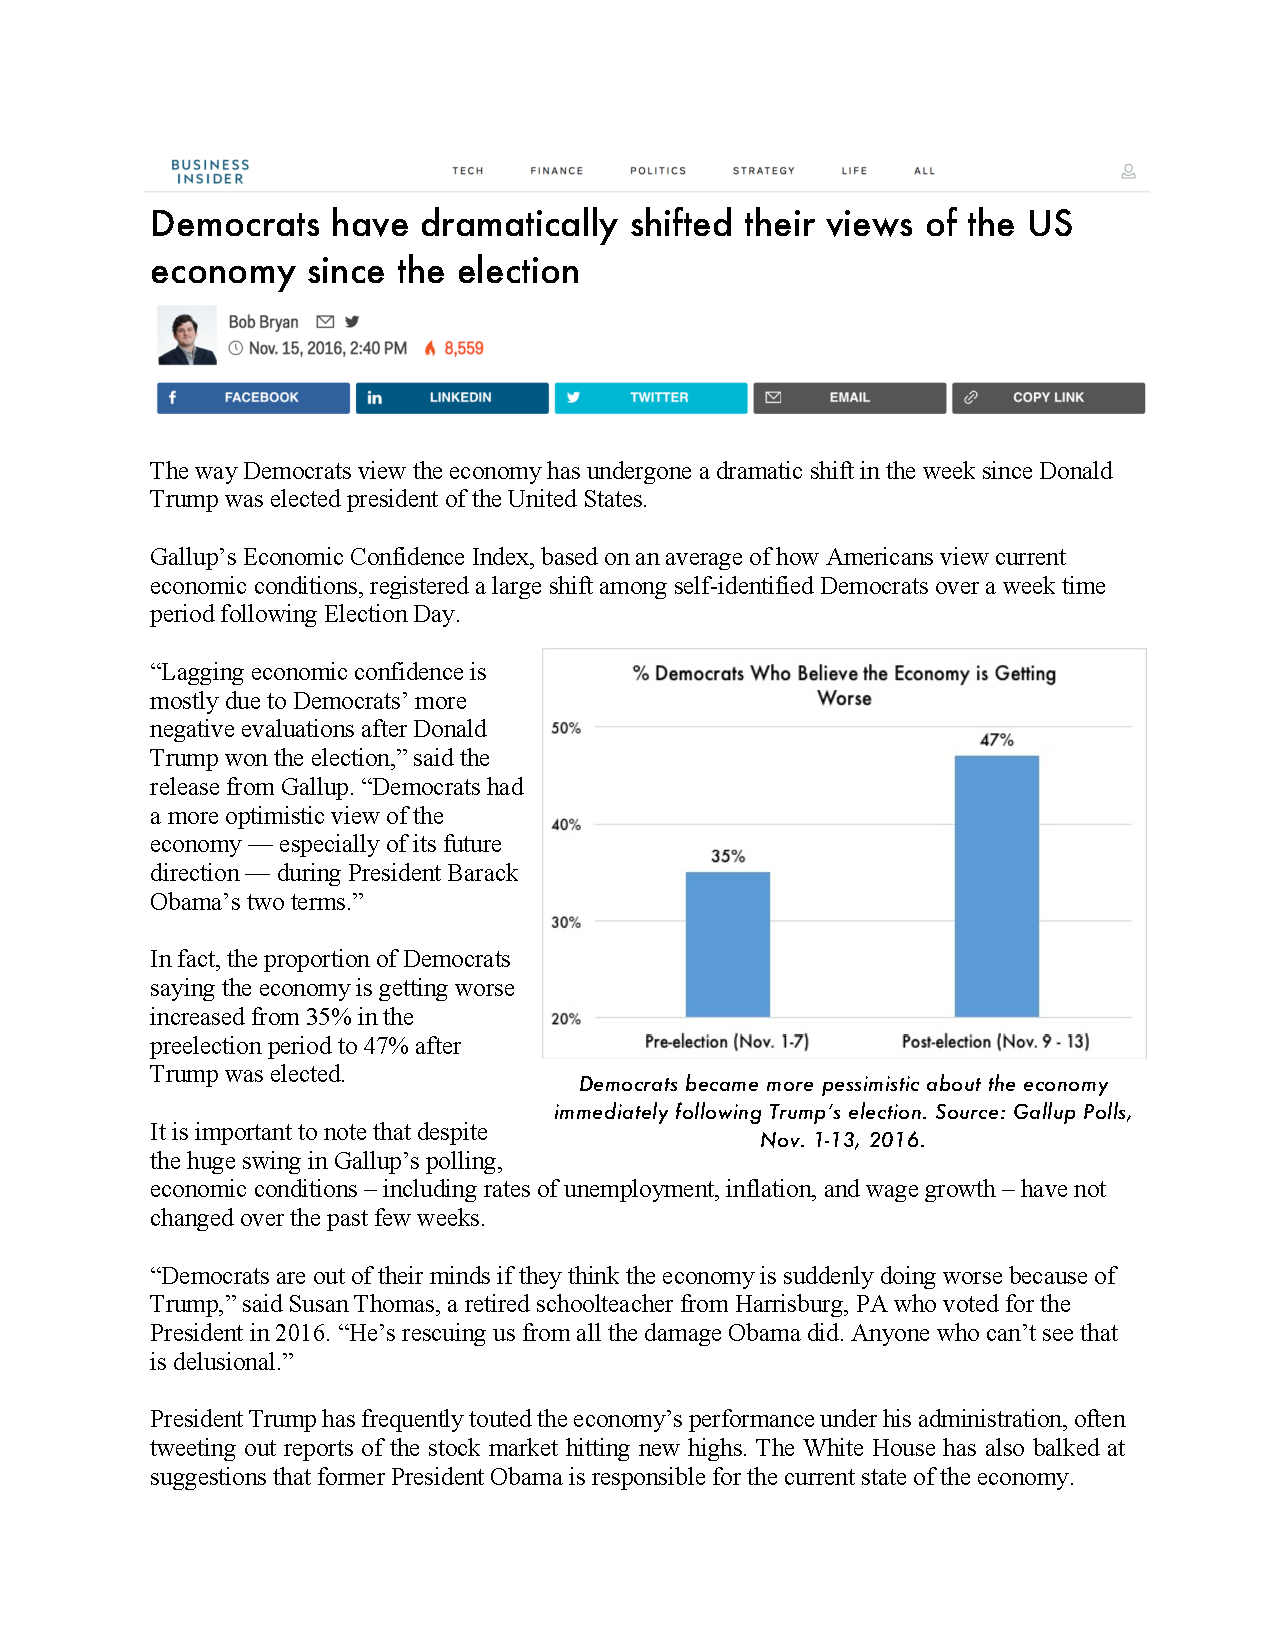
\includegraphics[width=1.05\textwidth]{dem_motivate.pdf}
\label{fig:minipage1}
\end{minipage}
\quad
\begin{minipage}[b]{0.45\linewidth}
\caption{Republican Bias}
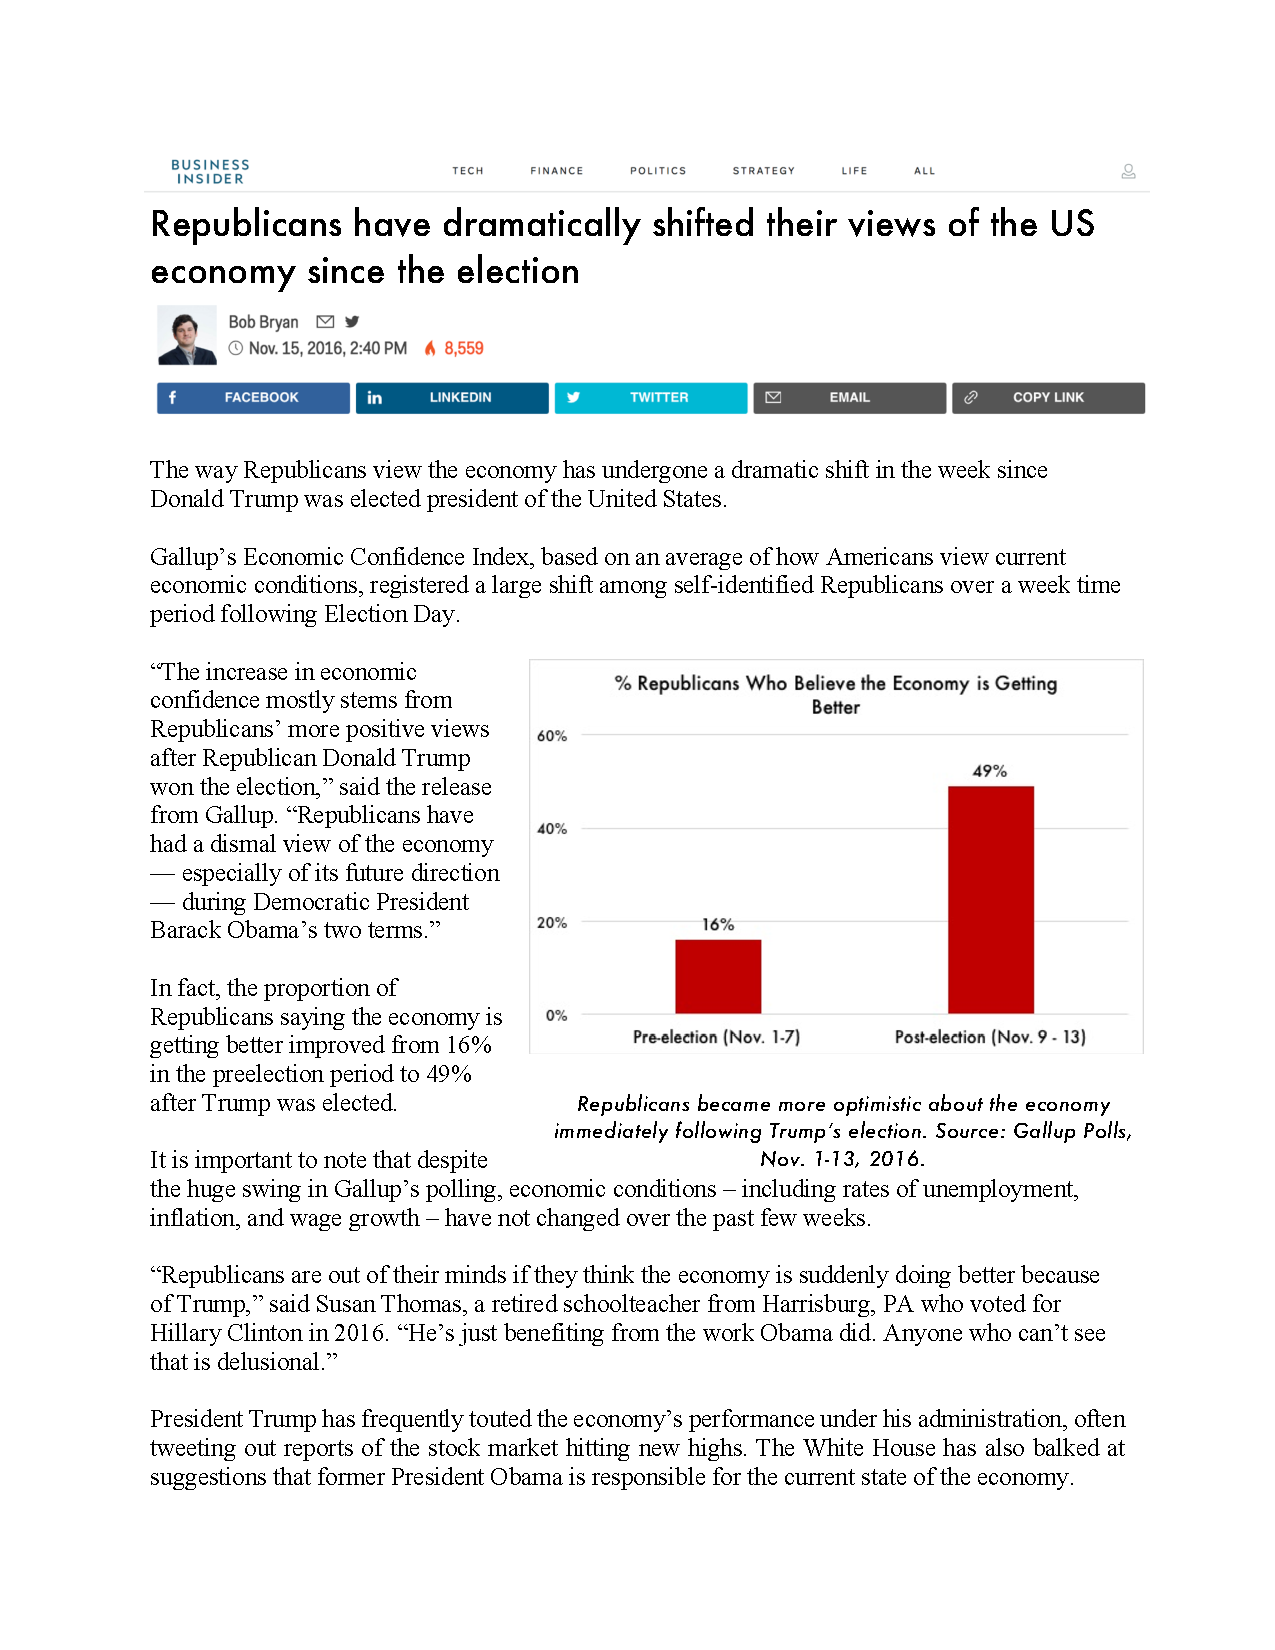
\includegraphics[width=1.05\textwidth]{rep_motivate.pdf}
\label{fig:minipage2}
\end{minipage}
\end{figure}


\end{document}